%\documentclass{article}
%\documentclass[journal]{IEEEtran}
%\documentclass[letterpaper, twoside, openright]{report}
%\documentclass{ActaOulu}
%\documentclass[12pt, twoside]{memoir}

%%%---%%%---%%%---%%%---%%%---%%%---%%%---%%%---%%%---%%%---%%%---%%%---%%%

\documentclass[11pt,a4paper,oldfontcommands]{memoir}
\usepackage[utf8]{inputenc}
\usepackage[T1]{fontenc}
\usepackage{microtype}
\usepackage{times}

\usepackage[
breaklinks=true,colorlinks=true,
%linkcolor=blue,urlcolor=blue,citecolor=blue,% PDF VIEW
linkcolor=black,urlcolor=black,citecolor=black,% PRINT
bookmarks=true,bookmarksopenlevel=2]{hyperref}

\usepackage{geometry}
% PDF VIEW
% \geometry{total={210mm,297mm},
% left=25mm,right=25mm,%
% bindingoffset=0mm, top=25mm,bottom=25mm}
% PRINT
\geometry{total={210mm,297mm},
left=20mm,right=20mm,
bindingoffset=10mm, top=25mm,bottom=25mm}

\OnehalfSpacing
%\linespread{1.3}

%%% CHAPTER'S STYLE
\chapterstyle{bianchi}
%\chapterstyle{ger}
%\chapterstyle{madsen}
%\chapterstyle{ell}
%%% STYLE OF SECTIONS, SUBSECTIONS, AND SUBSUBSECTIONS
\setsecheadstyle{\Large\bfseries\sffamily\raggedright}
\setsubsecheadstyle{\large\bfseries\sffamily\raggedright}
\setsubsubsecheadstyle{\bfseries\sffamily\raggedright}

%%% STYLE OF PAGES NUMBERING
%\pagestyle{companion}\nouppercaseheads 
%\pagestyle{headings}
%\pagestyle{Ruled}
\pagestyle{plain}
\makepagestyle{plain}
\makeevenfoot{plain}{\thepage}{}{}
\makeoddfoot{plain}{}{}{\thepage}
\makeevenhead{plain}{}{}{}
\makeoddhead{plain}{}{}{}


\maxsecnumdepth{subsection} % chapters, sections, and subsections are numbered
\maxtocdepth{subsection} % chapters, sections, and subsections are in the Table of Contents


%%%---%%%---%%%---%%%---%%%---%%%---%%%---%%%---%%%---%%%---%%%---%%%---%%%


\usepackage{color}
\usepackage[usenames,dvipsnames]{xcolor}
\usepackage{graphicx}
\usepackage{rotating}
\usepackage{float}
\graphicspath{ {figures/ASUDS_block_diagram(s)_5-2-2015/} }
\usepackage{caption}
\usepackage{subcaption}
\usepackage{array}
\usepackage{authblk}
\usepackage{mathtools}
\usepackage{url}
\usepackage{hyperref}
\hypersetup{colorlinks=true, filecolor=blue, citecolor=red, linkcolor=blue, urlcolor=RoyalBlue, bookmarks=true}

\setcounter{tocdepth}{4}
\setcounter{secnumdepth}{4}

%%%---%%%---%%%---%%%---%%%---%%%---%%%---%%%---%%%---%%%---%%%---%%%---%%%


\begin{document}

\title{Ultrasonics Spectrometer Code Manual}
\author{Matthew Rothfuss\thanks{\href{mailto:mrengr@ksu.edu}{mrengr@ksu.edu}, \href{mailto:mrengr@phys.ksu.edu}{mrengr@phys.ksu.edu}}}
\affil{Department of Animal Science and Food Industry, Kansas State University}

\maketitle
\newpage
\tableofcontents
\newpage
\listoffigures
\listoftables

\chapter{LabView Basics}

\section{Introduction}

LabVIEW	(short	for	\textbf{Lab}oratory	\textbf{V}irtual	\textbf{I}nstrumentation	\textbf{E}ngineering	\textbf{W}orkbench) is a development environment for visual programming, developed by National Instruments (\href{http://www.ni.com/}{www.ni.com}). The code files (or program files) are identified by the \textbf{.vi} extension called \textbf{Virtual Instruments} or \textbf{VIs} for short. This graphical language is most commonly used for data acquisition, instrument control, signal processing (analysis), industrial automation, and more.

The next section will cover some basics of LabVIEW design and operation. For additional resources, the current (2013) LabVIEW Getting Started Manual is located \href{http://www.ni.com/pdf/manuals/373427j.pdf}{here}.

\subsection{Additional Resources}

\cite{gomez_alvarez-arenas_air-coupled_2003}

\chapter{Theory of Operation}

Define the background concepts of how/what this program is accomplishing.  Make refs to papers but don't do the math here (don't have time for that).  Just outline the basics of what we want to do, what goes into the system, what the system does (ref manuals and such for theory \& papers), and what the system outputs.

\chapter{Code Structure}

Theory of code operation goes here. ie case structure, state machine, 

\section{Main VI}

Define the outline of the Main VI (the main program) and hit on each part of it.  Don't spend time explaining the subvi's here since i'm doing that in the \textbf{Custom VI's} section. Make sure to to be thorough on all the code that is not included in the subvi section.

The main program \textbf{ASUDS\_v13.vi} is contained within a Project file called \textcolor{red}{(file name here)}. When the program is ran it will first load the auto generated system settings files (via the LC931C\_Read.vi [\ref{fig:LC931C_Read_main}] or DPR300\_Read.vi) [\ref{tab:jsr}]) from the last time the program ran. A set of default system settings files are included for first time use. Next the Oscilloscope and the JSR are both initialized via LC931C\_Int.vi and DPR300\_Int.vi [\ref{tab:osc}, \ref{tab:jsr}] with the loaded settings as-well-as set the front panel controls to the loaded settings. At the same time any leftover front panel controls are set to their default values and all block diagram cases are set to there initial positions.

Once the settings clusters have been set properly and

\section{Custom VI's}

List of custom VI's and a short description of what they do. In the next section we will take a deeper look into each of these subvi's.

These files load in most of the front panel controls, some are missing since more code has been added but the vi that saves the system settings has not been updated to include the new additions.

\subsection{Oscilloscope VIs}

\begin{table}[H]
	\centering
	\begin{tabular}{ m{2.5cm} | m{5cm} | m{5cm} }
		\hline
		\hline \multicolumn{3}{c}{Oscilloscope} \\ \hline \hline
		VI & File Name & Description \\ \hline
		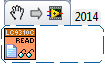
\includegraphics[scale=0.625]{LC931C_Read_main} & \hyperref[LC9310C_Read]{LC9310C\_Read.vi} & Load Oscilloscope Setting from System Generated File \\ \hline
		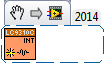
\includegraphics[scale=0.625]{LC931C_Int_main_02} & \hyperref[LC9310C_Int]{LC9310C\_Int.vi} & Initialize Oscilloscope Settings \\ \hline
		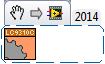
\includegraphics[scale=0.625]{LC931C_settings_main_01} & \hyperref[LC9310C_settings]{LC9310C\_settings.vi} & Apply Settings to Oscilloscope \\ \hline
		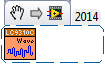
\includegraphics[scale=0.625]{LC931C_single-wave-output_main_01} & \hyperref[LC9310C_swo]{LC9310C\_single-wave-output.vi} & Acquire Single Wave from Oscilloscope and Average \\ \hline
		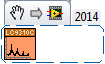
\includegraphics[scale=0.625]{LC931C_norm-pad-hilbert_main_01} & \hyperref[LC9310C_nph]{LC9310C\_norm-pad-hilbert.vi} & Oscilloscope Tab Settings \\ \hline
		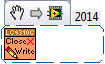
\includegraphics[scale=0.625]{LC931C-Config-Write-Close_main_01} & \hyperref[LC9310C_cwc]{LC9310C-Config-Write-Close.vi} & Write Oscilloscope settings to System File and close Oscilloscope resources \\ \hline
	\end{tabular}
	\caption{Oscilloscope Custom VIs}
	\label{tab:osc}
\end{table}

\subsubsection{LC9310C\_Read.vi} \label{LC9310C_Read}
\noindent\hrulefill

\begin{figure}[h]
	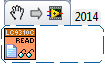
\includegraphics[scale=0.625]{LC931C_Read_main}
	\label{fig:LC9310C_Read_main}
\end{figure}

The LC931C\_Read.vi reads the LeCroy 9310C oscillosope settings from file and loads the values into a \textbf{LeCroy 9310C Settings} cluster. The settings folder (\textbf{System\_Settings}) is located in the root directory of the main VI. This VI requires the \href{http://sine.ni.com/nips/cds/view/p/lang/en/nid/209753}{MGI Library}. Figure (\ref{fig:LC9310C_Read_blkdig}) is the block diagram.  It is setup as an error case structure. When an error is detected from the \textbf{error (in)} input then the code in the green box does not execute and the \textbf{LeCroy 9310C Settings} cluster outputs a set of default values.

The for loop steps through each list section of the ".ini" file. Each list section corresponds to one of the input cluster constants \textit{(LC930x\_TimeBase, LC930x\_Vertical\_Setup, LC930x\_Trigger\_Edge\_Setup, LC930x\_Read\_Wave)}. The \textbf{MGI Read Anything} VI needs to know the format of each section. This is accomplished by the cluster constants being converted into variants for the Read Anything variant input.  For more on the MGI VI's and how they operate, refer to their help manuals respectively. Once the \textbf{MGI Read Anything} VI has pulled out the relevant data, then the \textbf{variant to data} vi is used to reformat the output back to the cluster constant. The output for each cluster only executes when its section is read (hence when integer counter =0. =1, =2, =3, then data is outputted). 

\noindent\hrulefill\, \hyperref[tab:osc]{Back to Osc.\ Table \ref{tab:osc}}

\begin{sidewaysfigure}[p!]
	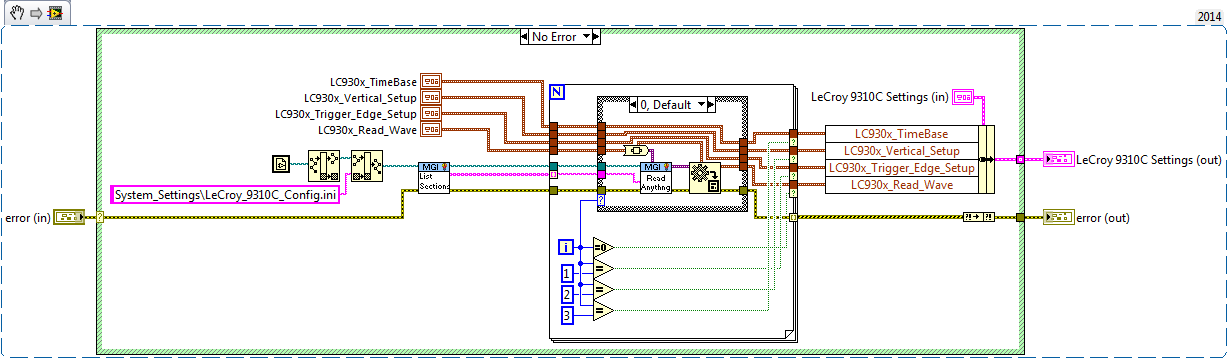
\includegraphics[width=\textheight,keepaspectratio]{LC931C_Read_blockdiagram}
	\caption{LC9310C\_Read.vi}
	\label{fig:LC9310C_Read_blkdig}
	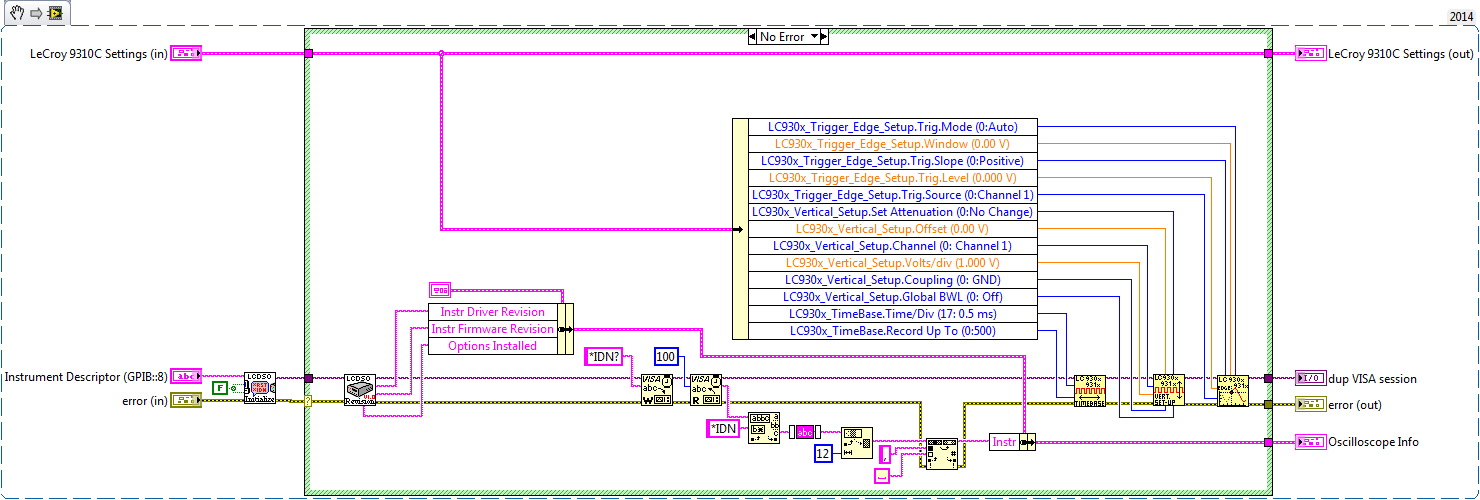
\includegraphics[width=\textheight,keepaspectratio]{LC931C_Int_blockdiagram}
	\caption{LC9310C\_Int.vi}
	\label{fig:LC9310C_Int_blkdig}
\end{sidewaysfigure}

\subsubsection{LC9310C\_Int.vi} \label{LC9310C_Int}
\noindent\hrulefill

\begin{figure}[h]
	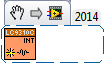
\includegraphics[scale=0.625]{LC931C_Int_main_02}
	\label{fig:LC9310C_Int_main_02}
\end{figure}

The LC931C\_Int.vi initializes the LeCroy 9310C Oscilloscope settings: \textit{trigger setup, vertical setup, and time setup (horizontal)}. This VI requires the \href{http://sine.ni.com/apps/utf8/niid_web_display.download_page?p_id_guid=E3B19B3E9608659CE034080020E74861}{LeCroy lc930x1x Library}. Figure (\ref{fig:LC9310C_Int_blkdig}) is the block diagram.  It is setup as an error case structure. When an error is detected from the \textit{error (in)} input then the code in the green box does not execute, instead the case not shown passes through the \textbf{LeCroy 9310C Settings} unchanged.

The \textbf{LCDSO Initialize} VI takes the GPIB location of the oscilloscope and creates a duped VISA session for the instrument. Next the \textbf{LCDSO Revision} reads the instruments Driver, Firmware, and Options Installed. All are put into a cluster called \textbf{Oscilloscope Info}, but first we write to the VISA session \textit{*IND?} an identification command. Next read the response with a count of 100 (the length of our expected response), this will give an identification string that is placed into the \textbf{Oscilloscope Info} cluster.

From the \textbf{LeCroy 9310C Settings} in cluster we set the \textbf{LC930x TimeBase}, \textbf{LC930x Vertical Setup}, and \textbf{LC930x Trigger} VIs. The cluster is unbundled and each setting is routed to it's respective input. Note the \textbf{LeCroy 9310C Settings} cluster is just passed through in this VI and not altered, because it is only pulling out data to setup other VIs.

\noindent\hrulefill\, \hyperref[tab:osc]{Back to Osc.\ Table \ref{tab:osc}}

\subsubsection{LC9310C\_Settings.vi} \label{LC9310C_settings}
\noindent\hrulefill

\begin{figure}[h]
	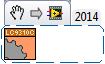
\includegraphics[scale=0.625]{LC931C_settings_main_01}
	\label{fig:LC9310C_settings_main_01}
\end{figure}

The LC931C\_Settings.vi applies changes to the \textit{trigger setup, vertical setup, and time setup (horizontal)} oscilloscope VIs. This VI requires the \href{http://sine.ni.com/apps/utf8/niid_web_display.download_page?p_id_guid=E3B19B3E9608659CE034080020E74861}{LeCroy lc930x1x Library}. Figure (\ref{fig:LC9310C_settings_blkdig_01}) is the block diagram. On the "error" case the \textbf{LeCroy 9310C Settings} cluster is passed through and so is the error cluster.

\noindent\hrulefill\, \hyperref[tab:osc]{Back to Osc.\ Table \ref{tab:osc}}

\begin{figure}[H]
	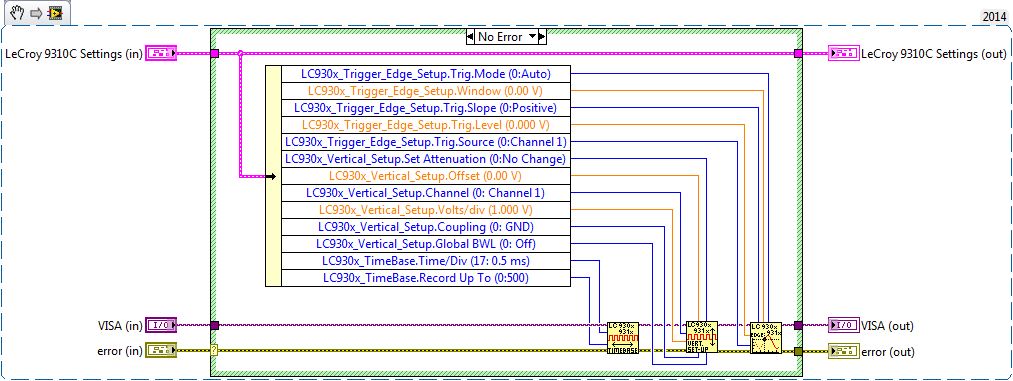
\includegraphics[width=\textwidth,keepaspectratio]{LC931C_settings_blockdiagram_01}
	\caption{LC9310C\_Settings.vi}
	\label{fig:LC9310C_settings_blkdig_01}
\end{figure}

\subsubsection{LC9310C\_Single-Wave-Output.vi} \label{LC9310C_swo}
\noindent\hrulefill

\begin{figure}[H]
	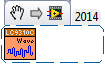
\includegraphics[scale=0.625]{LC931C_single-wave-output_main_01}
	\label{fig:LC9310C_single-wave-output_main_01}
\end{figure}

The LC931C\_Single-Wave-Output.vi acquires the signal from the LeCroy 9310C Oscilloscope and will average the acquired wave according to the desired sample size. This VI requires the \href{http://sine.ni.com/apps/utf8/niid_web_display.download_page?p_id_guid=E3B19B3E9608659CE034080020E74861}{LeCroy lc930x1x Library}. Figure (\ref{fig:LC9310C_Int_blkdig}) is the block diagram.  It is setup as an error case structure. When an error is detected from the \textit{error (in)} input then the code in the green box does not execute, instead the case not shown passes through the \textbf{LeCroy 9310C Settings}, \textbf{VISA (in)}, and \textbf{error (in)} unchanged. The \textbf{Wave Output} cluster will reset to an empty Waveform cluster during an error.

We first initialize an empty array with the size of our acquired wave from the \textbf{LCDSO Simple Read} VI. Take the Source channel setting from the \textbf{LeCroy 9310C Settings} cluster and set both \textbf{LCDSO Simple Read} VIs. The for loop is setup to first add all the arrays together (\hyperref[subfig:LC931C_single-wave-output_blkdig_02]{Figure \ref{subfig:LC931C_single-wave-output_blkdig_02}}) and then once the for loop indices indicator and the number of times the loop has ran match, then the added array is divided by total number of samples and placed back into the \textbf{Wave Output} cluster. (\hyperref[subfig:LC931C_single-wave-output_blkdig_01]{Figure \ref{subfig:LC931C_single-wave-output_blkdig_01}}) If no averaging is needed because the sample size is 1, meaning average over one sample (need 2 to average), then the for loop will run once and the \textbf{Wave Output} cluster will be passed out. (\hyperref[subfig:LC931C_single-wave-output_blkdig_03]{Figure \ref{subfig:LC931C_single-wave-output_blkdig_03}})

\noindent\hrulefill\, \hyperref[tab:osc]{Back to Osc.\ Table \ref{tab:osc}}

\begin{sidewaysfigure}[p!]
	\begin{subfigure}[t]{\textheight}
		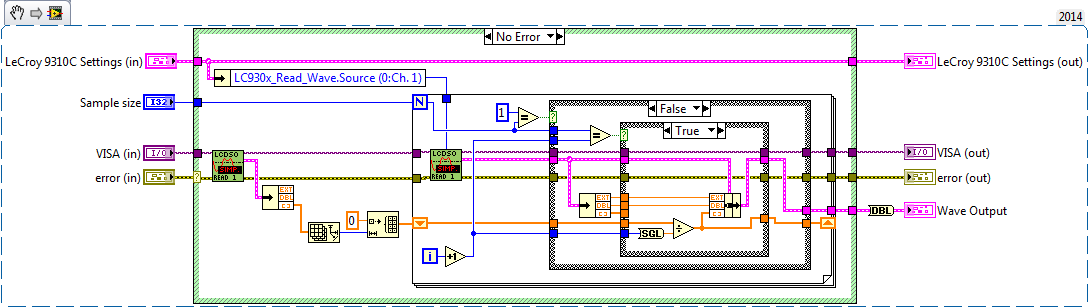
\includegraphics[width=\textheight,keepaspectratio]{LC931C_single-wave-output_blockdiagram_01}
		\caption{Overall Code with Outer Case False \& Inner Case True}
		\label{subfig:LC931C_single-wave-output_blkdig_01}
	\end{subfigure}%
	\vspace{1cm}
	\begin{subfigure}[t]{0.5\textheight}
		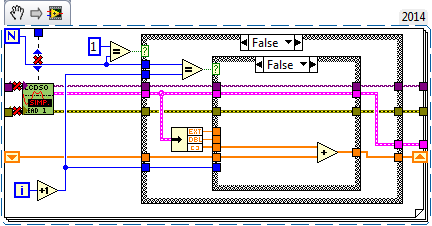
\includegraphics[width=0.45\textheight,keepaspectratio]{LC931C_single-wave-output_blockdiagram_02}
		\caption{Both Cases False}
		\label{subfig:LC931C_single-wave-output_blkdig_02}
	\end{subfigure}
	\begin{subfigure}[t]{0.5\textheight}
		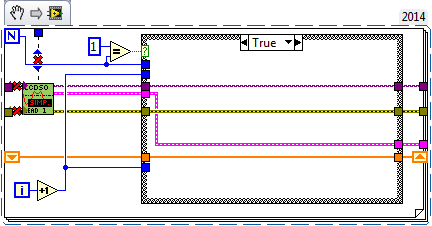
\includegraphics[width=0.45\textheight,keepaspectratio]{LC931C_single-wave-output_blockdiagram_03}
		\caption{Outer Case True}
		\label{subfig:LC931C_single-wave-output_blkdig_03}
	\end{subfigure}
	\caption{LC9310C\_single-wave-output.vi}
	\label{fig:LC9310C_single-wave-output_blkdig-all}
\end{sidewaysfigure}

\subsubsection{LC9310C\_Norm-Pad-Hilbert.vi} \label{LC9310C_nph}
\noindent\hrulefill

\begin{figure}[H]
	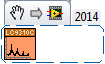
\includegraphics[scale=0.625]{LC931C_norm-pad-hilbert_main_01}
	\label{fig:LC9310C_norm-pad-hilbert_main_01}
\end{figure}

The LC931C\_Norm-Pad-Hilbert.vi will Pad the Y-Array with Zeros on both sides, Normalize the Y-Array, and apply a Fast Hilbert Transform on the waveform cluster. This VI requires the \textbf{U-Sonic Hilbert Transform} VI. Figure (\ref{fig:LC9310C_norm-pad-hilber_blkdig}) is the block diagram.  It is setup as an error case structure. When an error is detected from the \textit{error (in)} input then the code in the green box does not execute, instead the case not shown passes through the \textbf{LeCroy 9310C Settings}, \textbf{VISA (in)}, \textbf{Wave Input}, and \textbf{error (in)} unchanged.

The far left case applies the option to pad both sides of the Y-Array with zeros. This is done by pulling out the array from the \textbf{Wave Input} cluster, reversing it and applying the Pad with zeros subVI. Then reverse the array again to apply the zero pad on the other end of the array. The padded array is then rebundled into the \textbf{Wave Input} cluster.

The middle case was meant to normalize the Y-Array, but the way it is currently setup is incorrect. There are different ways to normalize a signal and each have a slightly different reason for doing so. If normalization is needed then remove the Mean VI and just pass through the normalized signal.

The far right case applies a Fast Hilbert Transformation to the \textbf{Wave Input} cluster. This VI is based from the \href{http://www.ni.com/example/28618/en/}{Ultrasonic Non-destructive Testing Starter Kit} and was modified to accompany our code. This is used to help view the oscilloscope signal but is not used it the process of data acquisition.

\noindent\hrulefill\, \hyperref[tab:osc]{Back to Osc.\ Table \ref{tab:osc}}

\begin{sidewaysfigure}[p!]
	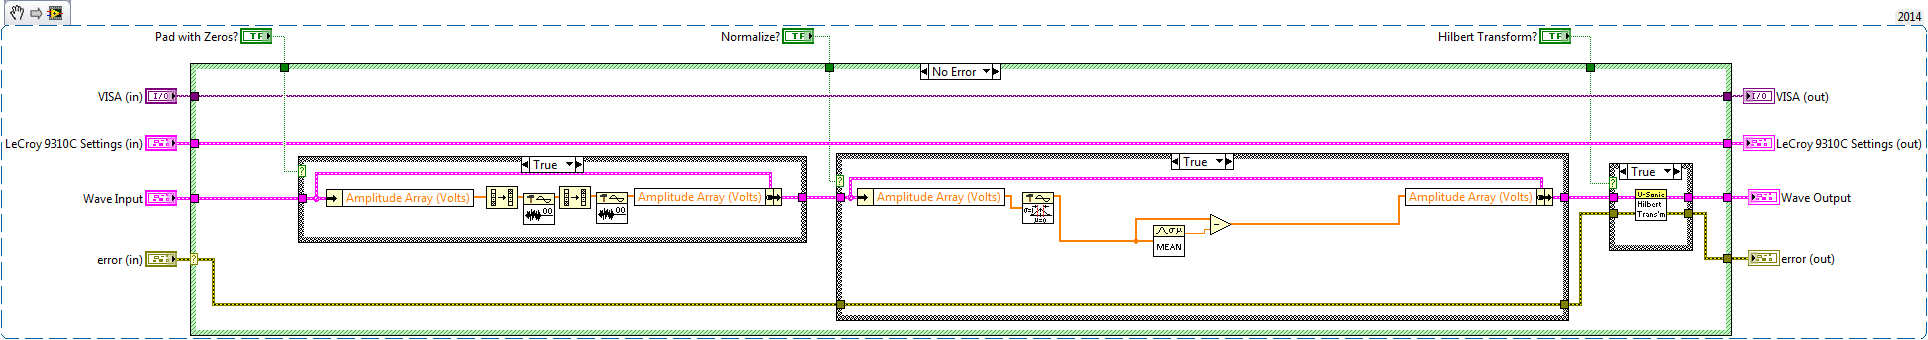
\includegraphics[width=\textheight,keepaspectratio]{LC931C_norm-pad-hilbert_blockdiagram_01}
	\caption{LC9310C\_Norm-Pad-Hilbert.vi}
	\label{fig:LC9310C_norm-pad-hilber_blkdig}
	\vspace{2cm}
	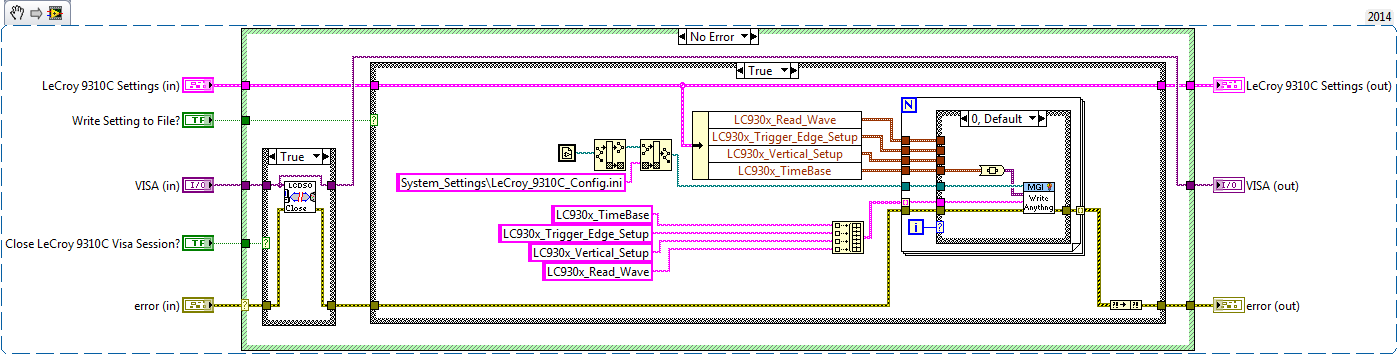
\includegraphics[width=\textheight,keepaspectratio]{LC931C-Config-Write-Close_blockdiagram_01}
	\caption{LC9310C-Config-Write-Close.vi}
	\label{fig:LC9310C-Config-Write-Closet_blkdig}
\end{sidewaysfigure}

\subsubsection{LC9310C-Config-Write-Close.vi} \label{LC9310C_cwc}
\noindent\hrulefill

\begin{figure}[H]
	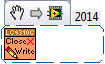
\includegraphics[scale=0.625]{LC931C-Config-Write-Close_main_01}
	\label{fig:LC9310C-Config-Write-Close_main_01}
\end{figure}

The LC9310C-Config-Write-Close.vi closes (releases) the oscilloscope VISA session and writes the \textbf{LeCroy 9310C Settings} cluster to the system settings file (located in the folder (\textbf{System\_Settings}) which is in the root directory of the main VI) to be loaded by the LC9310C\_Read.vi the next time the program is ran. This VI requires the \href{http://sine.ni.com/nips/cds/view/p/lang/en/nid/209753}{MGI Library}. Figure (\ref{fig:LC9310C-Config-Write-Close_blkdig}) is the block diagram.  It is setup as an error case structure. When an error is detected from the \textit{error (in)} input then the code in the green box does not execute.

The left case structure closes the oscilloscope VISA session. The right case structure pulls out the clusters \textit{(LC930x\_TimeBase, LC930x\_Vertical\_Setup, LC930x\_Trigger\_Edge\_Setup, LC930x\_Read\_Wave)} and places then in the system settings configuration file \textit{LeCroy\_9310C\_Config.ini}. By default both of these case structures are set to True.

The \textbf{MGI Write Anything} VI takes the information from each cluster and places in to a section, named by the four strings built into an array, located at the file path input.

\textbf{Note:} It is important that the VISA session be closed and not left open. If left open, then the next time the program is ran the oscilloscope VIs may return an error. This happens because LabVIEW still thinks a device is connected to that VISA session, but it's not because VISA sessions are tied to the process ID of the LabVIEW program. Meaning each time a program is ran, it runs under a different ID so the VISA sessions don't overlap. 

\noindent\hrulefill\, \hyperref[tab:osc]{Back to Osc.\ Table \ref{tab:osc}}

\begin{sidewaysfigure}[p!]
	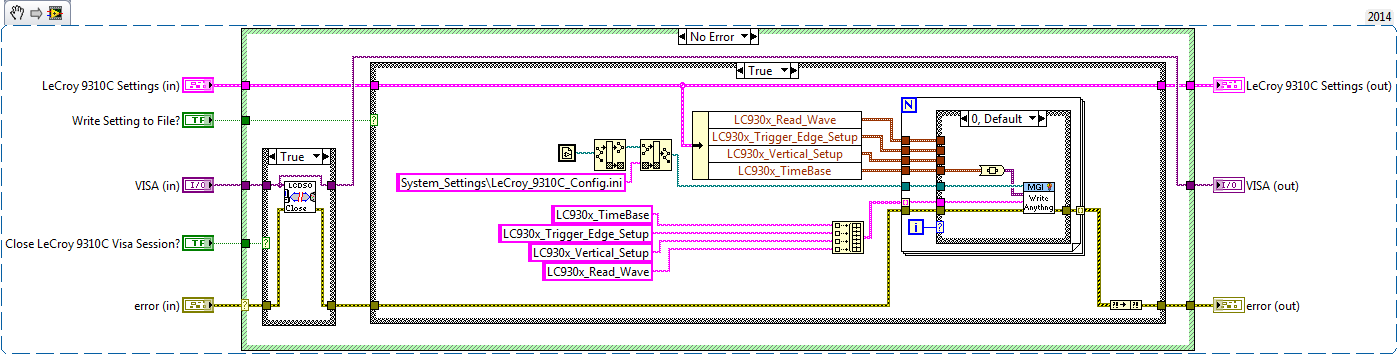
\includegraphics[width=\textheight,keepaspectratio]{LC931C-Config-Write-Close_blockdiagram_01}
	\caption{LC9310C-Config-Write-Close.vi}
	\label{fig:LC9310C-Config-Write-Close_blkdig}
\end{sidewaysfigure}

\newpage

\subsection{JSR Pulser/Receiver VIs}

\begin{table}[H]
	\centering
	\begin{tabular}{ m{2.5cm} | m{5cm} | m{5cm} }
		\hline
		\hline \multicolumn{3}{c}{JSR Pulser/Receiver} \\ \hline \hline
		VI & File Name & Description \\ \hline
		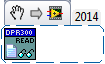
\includegraphics[scale=0.625]{DPR300_Read_main} & \hyperref[DPR300_Read]{DPR300\_Read.vi} & Load Pulser/Receiver Setting from System Generated File \\ \hline
		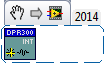
\includegraphics[scale=0.625]{DPR300_Int_main_02} & \hyperref[DPR300_Int]{DPR300\_Int.vi} & Initialize Pulser/Receiver Settings \\ \hline
		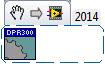
\includegraphics[scale=0.625]{DPR300_settings_main_01} & \hyperref[DPR300_settings]{DPR300\_settings.vi} & Apply Settings to Pulser/Receiver \\ \hline
		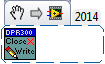
\includegraphics[scale=0.625]{DPR300-Config-Write-Close_main_01} & \hyperref[DPR300_cwc]{DPR300-Config-Write-Close.vi} & Write Pulser/Receiver settings to System File and close Pulser/Receiver resources \\ \hline
	\end{tabular}
	\caption{JSR Pulser/Receiver Custom VI's}
	\label{tab:jsr}
\end{table}

\subsubsection{DPR300\_Read.vi} \label{DPR300_Read}
\noindent\hrulefill

\begin{figure}[h]
	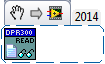
\includegraphics[scale=0.625]{DPR300_Read_main}
	\label{fig:DPR300_Read_main}
\end{figure}

The DPR300\_Read.vi reads the JSR DPR300 Pulser/Receiver settings from file and loads the values into a \textbf{DPR300 Settings} cluster. The settings folder (\textbf{System\_Settings}) is located in the root directory of the main VI. This VI requires the \href{http://sine.ni.com/apps/utf8/niid_web_display.download_page?p_id_guid=EE0D9BE18DD85923E0340003BA7CCD71}{MGI Library}. Figure (\ref{fig:DPR300_Read_blkdig}) is the block diagram.  It is setup as an error case structure. When an error is detected from the \textbf{error (in)} input then the code in the green box does not execute and the \textbf{DPR300 Settings} cluster outputs a set of default values.

The for loop steps through each list section of the ".ini" file. Each list section corresponds to one of the input cluster constants \textit{(DPR300\_Int\_Adress, DPR300\_PRF\_Settings, DPR300\_Generated\_Pulse, DPR300\_Received)}. The \textbf{MGI Read Anything} VI needs to know the format of each section. This is accomplished by the cluster constants being converted into variants for the Read Anything variant input. For more on the MGI VI's and how they operate, refer to their help manuals respectively. Once the \textbf{MGI Read Anything} VI has pulled out the relevant data, then the \textbf{variant to data} vi is used to reformat the output back to the cluster constant. The output for each cluster only executes when its section is read (hence when integer counter =0. =1, =2, =3, then data is outputted).

\noindent\hrulefill\, \hyperref[tab:jsr]{Back to JSR Table \ref{tab:jsr}}

\begin{sidewaysfigure}[p!]
	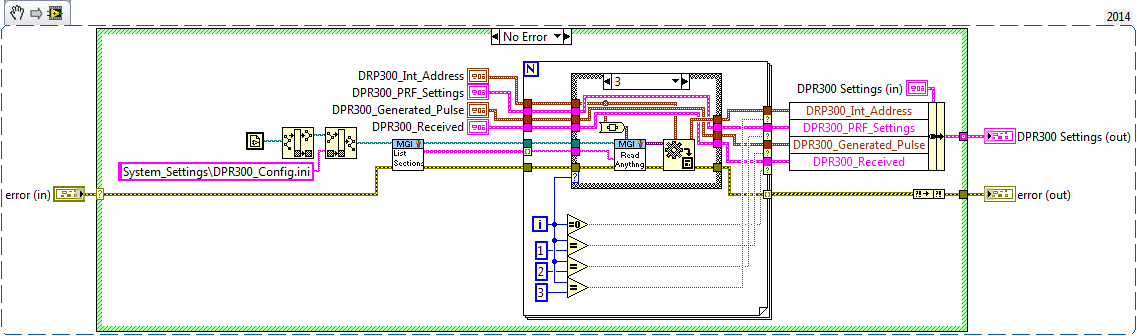
\includegraphics[width=\textheight,keepaspectratio]{DPR300_Read_blockdiagram}
	\caption{DPR300\_Read.vi}
	\label{fig:DPR300_Read_blkdig}
	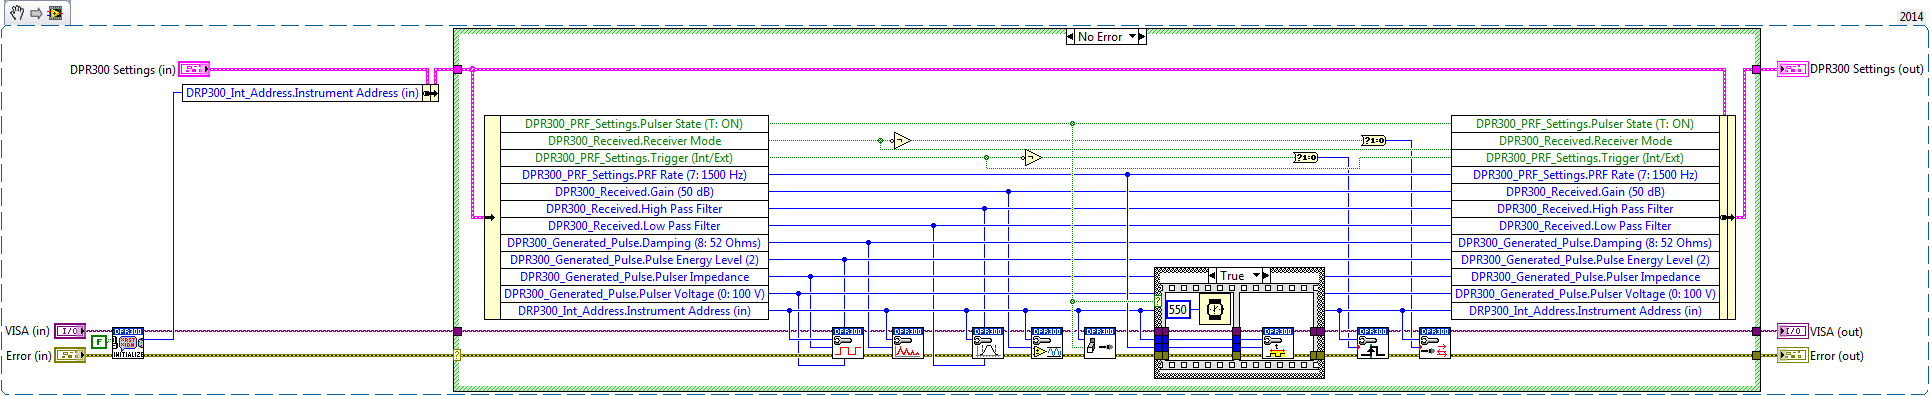
\includegraphics[width=\textheight,keepaspectratio]{DPR300_Int_blockdiagram_01}
	\caption{DPR300\_Int.vi}
	\label{fig:DPR300_Int_blkdig}
\end{sidewaysfigure}

\subsubsection{DPR300\_Int.vi} \label{DPR300_Int}
\noindent\hrulefill

\begin{figure}[h]
	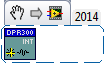
\includegraphics[scale=0.625]{DPR300_Int_main_02}
	\label{fig:DPR300_Int_main_02}
\end{figure}

The DPR300\_Int.vi initializes the JSR DPR300 Pulser/Receiver settings: \textit{generated pulse setup, dampening, low pass \& high pass filters, gain, pulser state (on/off), pulser repition frequency, trigger (Internal/External), and receiver mode (Internal/External)}. This VI requires the \href{http://sine.ni.com/apps/utf8/niid_web_display.download_page?p_id_guid=EE0D9BE18DD85923E0340003BA7CCD71}{JSR Ultrasonics dpr300 Library}. Figure (\ref{fig:DPR300_Int_blkdig}) is the block diagram.  It is setup as an error case structure. When an error is detected from the \textit{error (in)} input then the code in the green box does not execute, instead the case not shown passes through the \textbf{DPR300 Settings} and \textbf{error (in)} unchanged.

The \textbf{DPR300 Initialize} VI prepares JSR DPR300 Pulser/Receiver for use and identifies the instrument address which is then updated in the \textbf{DPR300 Settings} cluster. From there each value of the cluster is unbundled and sent to its respective VI. When the \textit{Pulser State} is set to true then a wait time is needed before the rate is applied. The t/f case structure after the pulser state VI will wait when $550 ms$ to apply the rate settings when true. During the false case there is no need for a wait time but we still need to update the rate settings in case later the Pulser is used.

\noindent\hrulefill\, \hyperref[tab:jsr]{Back to JSR Table \ref{tab:jsr}}

\subsubsection{DPR300\_Settings.vi} \label{DPR300_settings}
\noindent\hrulefill

\begin{figure}[h]
	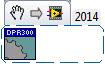
\includegraphics[scale=0.625]{DPR300_settings_main_01}
	\label{fig:DPR300_settings_main_01}
\end{figure}

The DPR300\_Settings.vi applies changes to the JSR DPR300 Pulser/Receiver settings: \textit{generated pulse setup, dampening, low pass \& high pass filters, gain, pulser state (on/off), pulser repition frequency, trigger (Internal/External), and receiver mode (Internal/External)}. This VI requires the \href{http://sine.ni.com/apps/utf8/niid_web_display.download_page?p_id_guid=EE0D9BE18DD85923E0340003BA7CCD71}{JSR Ultrasonics dpr300 Library}. Figure (\ref{fig:DPR300_set_blkdig}) is the block diagram.  It is setup as an error case structure. When an error is detected from the \textit{error (in)} input then the code in the green box does not execute, instead the case not shown passes through the \textbf{DPR300 Settings} and \textbf{error (in)} unchanged.

\noindent\hrulefill\, \hyperref[tab:jsr]{Back to JSR Table \ref{tab:jsr}}

\begin{sidewaysfigure}[p!]
	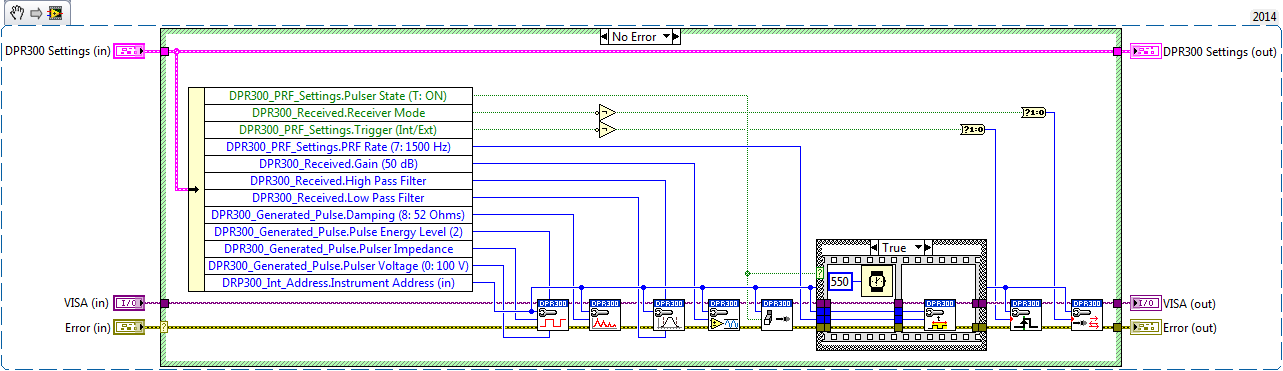
\includegraphics[width=\textheight,keepaspectratio]{DPR300_settings_blockdiagram_01}
	\caption{DPR300\_Settings.vi}
	\label{fig:DPR300_set_blkdig}
	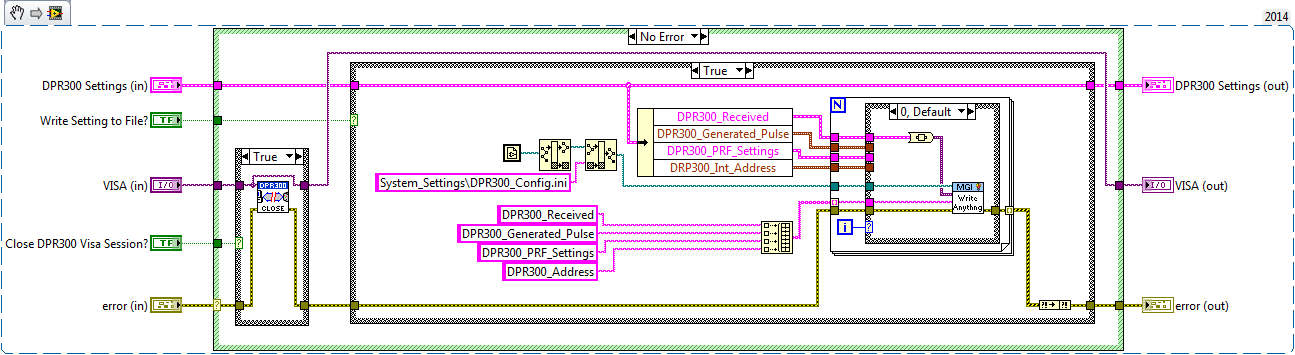
\includegraphics[width=\textheight,keepaspectratio]{DPR300-Config-Write-Close_blockdiagram_01}
	\caption{DPR300-Config-Write-Close.vi}
	\label{fig:DPR300_cwc_blkdig}
\end{sidewaysfigure}

\subsubsection{DPR300-Config-Write-Close.vi} \label{DPR300_cwc}
\noindent\hrulefill

\begin{figure}[h]
	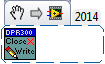
\includegraphics[scale=0.625]{DPR300-Config-Write-Close_main_01}
	\label{fig:DPR300-Config-Write-Close_main_01}
\end{figure}

The DPR300-Config-Write-Close.vi closes (releases) the JSR DPR300 Pulser/Receiver VISA session and writes the \textbf{DPR300 Settings} cluster to the system settings file (located in the folder (\textbf{System\_Settings}) which is in the root directory of the main VI) to be loaded by the DPR300\_Read.vi the next time the program is ran. This VI requires the \href{http://sine.ni.com/nips/cds/view/p/lang/en/nid/209753}{MGI Library}. Figure (\ref{fig:DPR300_cwc_blkdig}) is the block diagram.  It is setup as an error case structure. When an error is detected from the \textit{error (in)} input then the code in the green box does not execute and \textbf{DPR300 Settings} cluster, \textbf{VISA (in)}, and \textit{error (in)} are all passed through unchanged.

The left case structure closes the JSR DPR300 Pulser/Receiver VISA session. The right case structure pulls out the clusters \textit{(DPR300\_Received, DPR300\_Generated\_Pulse, DPR300\_PRF\_Settings, DPR300\_Address)} and places then in the system settings configuration file \textit{DPR300\_Config.ini}. By default both of these case structures are set to True.

The \textbf{MGI Write Anything} VI takes the information from each cluster and places it into a section, named by the four strings built into an array, located at the file path input.

\textbf{Note:} It is important that the VISA session be closed and not left open. If left open, then the next time the program is ran the oscilloscope VIs may return an error. This happens because LabVIEW still thinks a device is connected to that VISA session, but it's not because VISA sessions are tied to the process ID of the LabVIEW program. Meaning each time a program is ran, it runs under a different ID so the VISA sessions don't overlap.

\noindent\hrulefill\, \hyperref[tab:jsr]{Back to JSR Table \ref{tab:jsr}}

\newpage

\subsection{Ultrasonic Package VIs}

\begin{table}[H]
	\centering
	\begin{tabular}{ m{2.5cm} | m{5cm} | m{5cm} }
		\hline
		\hline \multicolumn{3}{c}{Ultrasonic Package} \\ \hline \hline
		VI & File Name & Description \\ \hline
		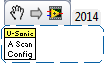
\includegraphics[scale=0.625]{USonic-A-Scan-Config-edit_main_01} & \hyperref[USonic-Config]{USonic-A-Scan-Config-edit.vi} & Configure/Set Gates for Data Acquisition \\ \hline
		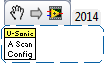
\includegraphics[scale=0.625]{USonic-A-Scan-Config-edit_main_01} & \hyperref[USonic-Gates]{USonic-Gates-edit.vi} & Pull Out Relevant Data from Gates for Data Acquisition \\ \hline
		
\includegraphics[scale=0.625]{USonic-FFT_main_01} & \hyperref[USonic-FFT]{USonic-FFT.vi} & Process Gate For Quick Analysis \\ \hline
	\end{tabular}
	\caption{Ultrasonic A-Scan Customized Package VI's}
	\label{tab:usonic}
\end{table}

\subsubsection{USonic-A-Scan-Config-edit.vi} \label{USonic-Config}
\noindent\hrulefill

\begin{figure}[h]
	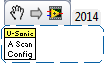
\includegraphics[scale=0.625]{USonic-A-Scan-Config-edit_main_01}
	\label{fig:USonic-A-Scan-Config-edit_main_01}
\end{figure}

The USonic-A-Scan-Config-edit.vi reads the \textbf {Gate Configuration} cluster and applies it to the \textbf{Data In} waveform cluster. It also finds the peak to peak time (time of fight). This VI was edited from the \href{http://www.ni.com/example/28618/en/}{Ultrasonic Non-destructive Testing Starter Kit} to fit our needs. The VI outputs the waveform cluster graph with the gates overlaid as-well-as it outputting the paired gate information for data analysis.

\noindent\hrulefill\, \hyperref[tab:usonic]{Back to USonic Table \ref{tab:usonic}}

\subsubsection{USonic-Gates-edit.vi} \label{USonic-Gates}
\noindent\hrulefill

\begin{figure}[h]
	
\includegraphics[scale=0.625]{USonic-FFT_main_01}
	\label{fig:USonic-Gates-edit_main_01}
\end{figure}

Pull Out Relevant Data from Gates for Data Acquisition. Don't have blockdiagram to look at right now, so will fill in this section later.

\noindent\hrulefill\, \hyperref[tab:usonic]{Back to USonic Table \ref{tab:usonic}}

\subsubsection{USonic-FFT.vi} \label{USonic-FFT}
\noindent\hrulefill

\begin{figure}[h]
	
\includegraphics[scale=0.625]{USonic-FFT_main_01}
	\label{fig:USonic-FFT_main_01}
\end{figure}

The USonic-FFT.vi takes the waveform data array and applies the single sided fast Fourier transform (FFT) which is a complex expression. From the complex expression the Magnitude and Phase are pulled out and have option associated with them. The VI outputs the FFT, Magnitude of FFT, and Phase of FFT as a waveform graph. Also the peak magnitude, peak phase and corresponding frequency are outputted for data analysis. Figure (\ref{fig:USonic-FFT-blkdig}) is the block diagram.  It is setup as an error case structure. When an error is detected from the \textit{error (in)} input then the code in the green box does not execute and all the outputs are set to zero while the error passes through.

The single sided fast Fourier transform VI takes the \textbf{Signal (V)} array and the \textbf{dt} double to computer the FFT and cut off one side of the FFT (thus the single sidedness). The output from the FFT is in frequency space so the \textbf{dt} now becomes \textbf{df} and the array output is now complex ($z=x+iy$). For just the FFT graph we take the complex array and \textbf{df} and rebuild the waveform for output. For the magnitude and phase we must convert the expression $z=x+iy$ to $z=r*\exp(i\theta)$ where $Magnitude=r^2$ (note the square, this is actually the power representation) and $phase=\theta$ (in rads). The true/false case structure for the FFT array gives the option to change the scaling of the array to decibel form. The true/false case structure for the phase gives the option to change the scaling to degrees as well as unwraps the phase array by eliminating discontinuities whose absolute values exceed either pi or 180.

Graphs are built as waveform clusters and originate from there respective arrays. For the math portion the processed magnitude array is built into a waveform and passed to the \textbf{Waveform Max/Min} VI to find the peak value ($y-axis$) and its corresponding frequency value ($x-axis$). The peak value is outputted as the Peak Magnitude of the Magnitude array and is feed into the \textbf{Search Array} VI that searches for the index (position in array) of the magnitude array. Then the index is used to pull out the corresponding element from the phase array, this in turn is the peak magnitude of the phase.

\noindent\hrulefill\, \hyperref[tab:usonic]{Back to USonic Table \ref{tab:usonic}}

\begin{figure}[H]
	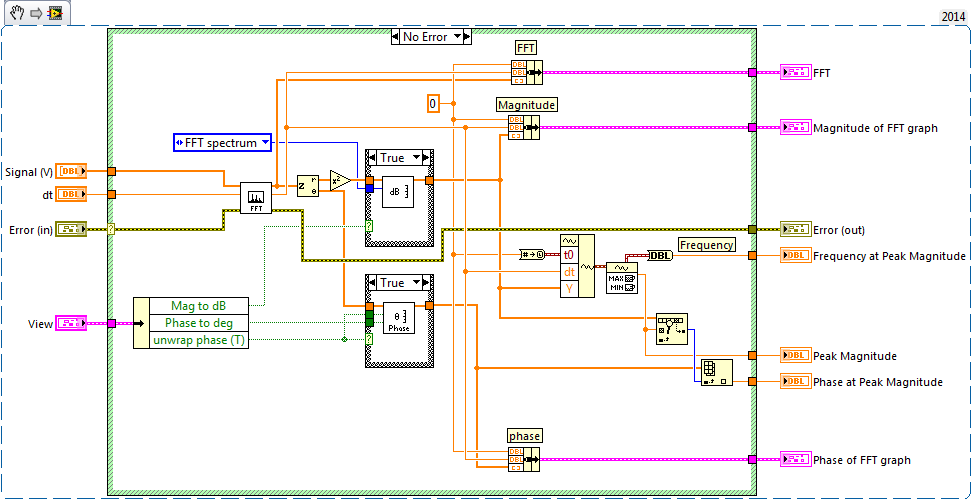
\includegraphics[width=\textwidth]{USonic-FFT_blockdiagram_01}
	\caption{USonic-FFT.vi}
	\label{fig:USonic-FFT-blkdig}
\end{figure}

\newpage

\subsection{Math VIs}

\begin{table}[H]
	\centering
	\begin{tabular}{ m {2.5cm} | m{5cm} | m{5cm} }
		\hline
		\hline \multicolumn{3}{c}{Math} \\ \hline \hline
		VI & File Name & Description \\ \hline
		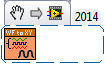
\includegraphics[scale=0.625]{Waveform-to-XY-Array_main_01} & \hyperref[Waveform-to-XY-Array]{Waveform-to-XY-Array.vi} & Convert Waveform to XY-Array \\ \hline
		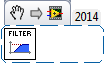
\includegraphics[scale=0.625]{Filter_signal_main_01} & \hyperref[Filter_signal]{Filter\_signal.vi} & Filter Wave Signal for Oscilloscope Tab (does not affect Data Acquisition) \\ \hline
		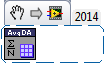
\includegraphics[scale=0.625]{Average-Dynamic-Array_main_01} & \hyperref[Average-Dynamic-Array]{Average-Dynamic-Array.vi} & Take the Average of N elements in a Dynamic Array \\ \hline
		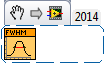
\includegraphics[scale=0.625]{FWHM-Poly_main_01} & \hyperref[FWHM-Poly]{FWHM-Poly.vi} & Compute the Full Width Half Max (FWHM) of either a Waveform, XY-Graph, or Waveform cluster \\ \hline
		\hline
	\end{tabular}
	\caption{Custom Math VI's}
	\label{tab:math}
\end{table}

\subsubsection{Waveform-to-XY-Array.vi} \label{Waveform-to-XY-Array}
\noindent\hrulefill

\begin{figure}[h]
	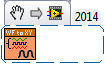
\includegraphics[scale=0.625]{Waveform-to-XY-Array_main_01}
	\label{fig:Waveform-to-XY-Array_main_01}
\end{figure}

The LC931C\_Read.vi reads the LeCroy 9310C oscillosope settings from file and loads the values into a \textbf{LeCroy 9310C Settings} cluster. The settings folder (\textbf{System\_Settings}) is located in the root directory of the main VI. This VI requires the \href{http://sine.ni.com/nips/cds/view/p/lang/en/nid/209753}{MGI Library}. Figure (\ref{fig:LC9310C_Read_blkdig}) is the block diagram.  It is setup as an error case structure. When an error is detected from the \textit{error (in)} input then the code in the green box does not execute.

The for loop steps through each list section of the ".ini" file. Each list section corresponds to one of the input cluster constants \textit{(LC930x\_TimeBase, LC930x\_Vertical\_Setup, LC930x\_Trigger\_Edge\_Setup, LC930x\_Read\_Wave)}. The \textbf{MGI Read Anything} VI needs to know the format of each section. This is accomplished by the cluster constants being converted into variants for the Read Anything variant input.  For more on the MGI VI's and how they operate, refer to their help manuals respectably. Once the \textbf{MGI Read Anything} VI has pulled out the relevant data, then the \textbf{variant to data} vi is used to reformat the output back to the cluster constant. The output for each cluster only executes when its section is read (hence the when integer counter =0. =1, =2, =3, then output data).

\noindent\hrulefill\, \hyperref[tab:math]{Back to Miscellaneous Table \ref{tab:math}}

\subsubsection{Filter\_signal.vi} \label{Filter_signal}
\noindent\hrulefill

\begin{figure}[h]
	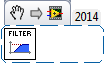
\includegraphics[scale=0.625]{Filter_signal_main_01}
	\label{fig:Filter_signal_main_01}
\end{figure}

The LC931C\_Read.vi reads the LeCroy 9310C oscillosope settings from file and loads the values into a \textbf{LeCroy 9310C Settings} cluster. The settings folder (\textbf{System\_Settings}) is located in the root directory of the main VI. This VI requires the \href{http://sine.ni.com/nips/cds/view/p/lang/en/nid/209753}{MGI Library}. Figure (\ref{fig:LC9310C_Read_blkdig}) is the block diagram.  It is setup as an error case structure. When an error is detected from the \textit{error (in)} input then the code in the green box does not execute.

The for loop steps through each list section of the ".ini" file. Each list section corresponds to one of the input cluster constants \textit{(LC930x\_TimeBase, LC930x\_Vertical\_Setup, LC930x\_Trigger\_Edge\_Setup, LC930x\_Read\_Wave)}. The \textbf{MGI Read Anything} VI needs to know the format of each section. This is accomplished by the cluster constants being converted into variants for the Read Anything variant input.  For more on the MGI VI's and how they operate, refer to their help manuals respectably. Once the \textbf{MGI Read Anything} VI has pulled out the relevant data, then the \textbf{variant to data} vi is used to reformat the output back to the cluster constant. The output for each cluster only executes when its section is read (hence the when integer counter =0. =1, =2, =3, then output data).

\noindent\hrulefill\, \hyperref[tab:math]{Back to Math Table \ref{tab:math}}

\subsubsection{Average-Dynamic-Array.vi} \label{Average-Dynamic-Array}
\noindent\hrulefill

\begin{figure}[h]
	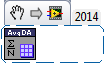
\includegraphics[scale=0.625]{Average-Dynamic-Array_main_01}
	\label{fig:Average-Dynamic-Array_main_01}
\end{figure}

The LC931C\_Read.vi reads the LeCroy 9310C oscillosope settings from file and loads the values into a \textbf{LeCroy 9310C Settings} cluster. The settings folder (\textbf{System\_Settings}) is located in the root directory of the main VI. This VI requires the \href{http://sine.ni.com/nips/cds/view/p/lang/en/nid/209753}{MGI Library}. Figure (\ref{fig:LC9310C_Read_blkdig}) is the block diagram.  It is setup as an error case structure. When an error is detected from the \textit{error (in)} input then the code in the green box does not execute.

The for loop steps through each list section of the ".ini" file. Each list section corresponds to one of the input cluster constants \textit{(LC930x\_TimeBase, LC930x\_Vertical\_Setup, LC930x\_Trigger\_Edge\_Setup, LC930x\_Read\_Wave)}. The \textbf{MGI Read Anything} VI needs to know the format of each section. This is accomplished by the cluster constants being converted into variants for the Read Anything variant input.  For more on the MGI VI's and how they operate, refer to their help manuals respectably. Once the \textbf{MGI Read Anything} VI has pulled out the relevant data, then the \textbf{variant to data} vi is used to reformat the output back to the cluster constant. The output for each cluster only executes when its section is read (hence the when integer counter =0. =1, =2, =3, then output data).

\noindent\hrulefill\, \hyperref[tab:math]{Back to Math Table \ref{tab:math}}

\subsubsection{FWHM-Poly.vi} \label{FWHM-Poly}
\noindent\hrulefill

\begin{figure}[h]
	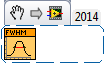
\includegraphics[scale=0.625]{FWHM-Poly_main_01}
	\label{fig:FWHM-Poly_main_01}
\end{figure}

The LC931C\_Read.vi reads the LeCroy 9310C oscillosope settings from file and loads the values into a \textbf{LeCroy 9310C Settings} cluster. The settings folder (\textbf{System\_Settings}) is located in the root directory of the main VI. This VI requires the \href{http://sine.ni.com/nips/cds/view/p/lang/en/nid/209753}{MGI Library}. Figure (\ref{fig:LC9310C_Read_blkdig}) is the block diagram.  It is setup as an error case structure. When an error is detected from the \textit{error (in)} input then the code in the green box does not execute.

The for loop steps through each list section of the ".ini" file. Each list section corresponds to one of the input cluster constants \textit{(LC930x\_TimeBase, LC930x\_Vertical\_Setup, LC930x\_Trigger\_Edge\_Setup, LC930x\_Read\_Wave)}. The \textbf{MGI Read Anything} VI needs to know the format of each section. This is accomplished by the cluster constants being converted into variants for the Read Anything variant input.  For more on the MGI VI's and how they operate, refer to their help manuals respectably. Once the \textbf{MGI Read Anything} VI has pulled out the relevant data, then the \textbf{variant to data} vi is used to reformat the output back to the cluster constant. The output for each cluster only executes when its section is read (hence the when integer counter =0. =1, =2, =3, then output data).

\noindent\hrulefill\, \hyperref[tab:math]{Back to Math Table \ref{tab:math}}

\newpage

\subsection{Miscellaneous VIs}

\begin{table}[H]
	\centering
	\begin{tabular}{ m {2.5cm} | m{5cm} | m{5cm} }
		\hline
		\hline \multicolumn{3}{c}{Miscellaneous} \\ \hline \hline
		VI & File Name & Description \\ \hline
		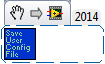
\includegraphics[scale=0.625]{Save-User-Config-File_main_01} & \hyperref[Save-User-Config-File]{Save-User-Config-File.vi} & Save all front panel controls to a user.ini settings file \\ \hline		
		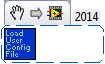
\includegraphics[scale=0.625]{Load-User-Config-File_main_01} & \hyperref[Load-User-Config-File]{Load-User-Config-File.vi} & Load the user.ini settings file \\ \hline
		\includegraphics[scale=0.625]{Time-Data_main_01} & \hyperref[Time-Data]{Time-Data.vi} & Load and Save Data Timing table \\ \hline
		\includegraphics[scale=0.625]{Instrument-error-handler_main_01} & \hyperref[IEH]{Instrument-error-handler.vi} & Pop-up error message for loss of Instrument signal\\ \hline
		\hline
	\end{tabular}
	\caption{Miscellaneous Custom VI's}
	\label{tab:misc}
\end{table}

\subsubsection{Save-User-Config-File.vi} \label{Save-User-Config-File}
\noindent\hrulefill

\begin{figure}[h]
	\includegraphics[scale=0.625]{Save-User-Config-File_main_01}
	\label{fig:Save-User-Config-File_main_01}
\end{figure}

The LC931C\_Read.vi reads the LeCroy 9310C oscillosope settings from file and loads the values into a \textbf{LeCroy 9310C Settings} cluster. The settings folder (\textbf{System\_Settings}) is located in the root directory of the main VI. This VI requires the \href{http://sine.ni.com/nips/cds/view/p/lang/en/nid/209753}{MGI Library}. Figure (\ref{fig:LC9310C_Read_blkdig}) is the block diagram.  It is setup as an error case structure. When an error is detected from the \textit{error (in)} input then the code in the green box does not execute.

The for loop steps through each list section of the ".ini" file. Each list section corresponds to one of the input cluster constants \textit{(LC930x\_TimeBase, LC930x\_Vertical\_Setup, LC930x\_Trigger\_Edge\_Setup, LC930x\_Read\_Wave)}. The \textbf{MGI Read Anything} VI needs to know the format of each section. This is accomplished by the cluster constants being converted into variants for the Read Anything variant input.  For more on the MGI VI's and how they operate, refer to their help manuals respectably. Once the \textbf{MGI Read Anything} VI has pulled out the relevant data, then the \textbf{variant to data} vi is used to reformat the output back to the cluster constant. The output for each cluster only executes when its section is read (hence the when integer counter =0. =1, =2, =3, then output data).

\noindent\hrulefill\, \hyperref[tab:misc]{Back to Misc.\ Table \ref{tab:misc}}

\subsubsection{Load-User-Config-File.vi} \label{Load-User-Config-File}
\noindent\hrulefill

\begin{figure}[h]
	\includegraphics[scale=0.625]{Load-User-Config-File_main_01}
	\label{fig:Load-User-Config-File_main_01}
\end{figure}

The LC931C\_Read.vi reads the LeCroy 9310C oscillosope settings from file and loads the values into a \textbf{LeCroy 9310C Settings} cluster. The settings folder (\textbf{System\_Settings}) is located in the root directory of the main VI. This VI requires the \href{http://sine.ni.com/nips/cds/view/p/lang/en/nid/209753}{MGI Library}. Figure (\ref{fig:LC9310C_Read_blkdig}) is the block diagram.  It is setup as an error case structure. When an error is detected from the \textit{error (in)} input then the code in the green box does not execute.

The for loop steps through each list section of the ".ini" file. Each list section corresponds to one of the input cluster constants \textit{(LC930x\_TimeBase, LC930x\_Vertical\_Setup, LC930x\_Trigger\_Edge\_Setup, LC930x\_Read\_Wave)}. The \textbf{MGI Read Anything} VI needs to know the format of each section. This is accomplished by the cluster constants being converted into variants for the Read Anything variant input.  For more on the MGI VI's and how they operate, refer to their help manuals respectably. Once the \textbf{MGI Read Anything} VI has pulled out the relevant data, then the \textbf{variant to data} vi is used to reformat the output back to the cluster constant. The output for each cluster only executes when its section is read (hence the when integer counter =0. =1, =2, =3, then output data).

\noindent\hrulefill\, \hyperref[tab:misc]{Back to Misc.\ Table \ref{tab:misc}}

\subsubsection{Time-Data.vi} \label{Time-Data}
\noindent\hrulefill

\begin{figure}[h]
	\includegraphics[scale=0.625]{Time-Data_main_01}
	\label{fig:Time-Data_main_01}
\end{figure}

The LC931C\_Read.vi reads the LeCroy 9310C oscillosope settings from file and loads the values into a \textbf{LeCroy 9310C Settings} cluster. The settings folder (\textbf{System\_Settings}) is located in the root directory of the main VI. This VI requires the \href{http://sine.ni.com/nips/cds/view/p/lang/en/nid/209753}{MGI Library}. Figure (\ref{fig:LC9310C_Read_blkdig}) is the block diagram.  It is setup as an error case structure. When an error is detected from the \textit{error (in)} input then the code in the green box does not execute.

The for loop steps through each list section of the ".ini" file. Each list section corresponds to one of the input cluster constants \textit{(LC930x\_TimeBase, LC930x\_Vertical\_Setup, LC930x\_Trigger\_Edge\_Setup, LC930x\_Read\_Wave)}. The \textbf{MGI Read Anything} VI needs to know the format of each section. This is accomplished by the cluster constants being converted into variants for the Read Anything variant input.  For more on the MGI VI's and how they operate, refer to their help manuals respectably. Once the \textbf{MGI Read Anything} VI has pulled out the relevant data, then the \textbf{variant to data} vi is used to reformat the output back to the cluster constant. The output for each cluster only executes when its section is read (hence the when integer counter =0. =1, =2, =3, then output data).

\noindent\hrulefill\, \hyperref[tab:misc]{Back to Misc.\ Table \ref{tab:misc}}

\subsubsection{Instrument-Error-Handler.vi} \label{IEH}
\noindent\hrulefill

\begin{figure}[h]
	\includegraphics[scale=0.625]{Instrument-error-handler_main_01}
	\label{fig:Instrument-error-handler_main_01}
\end{figure}

The LC931C\_Read.vi reads the LeCroy 9310C oscillosope settings from file and loads the values into a \textbf{LeCroy 9310C Settings} cluster. The settings folder (\textbf{System\_Settings}) is located in the root directory of the main VI. This VI requires the \href{http://sine.ni.com/nips/cds/view/p/lang/en/nid/209753}{MGI Library}. Figure (\ref{fig:LC9310C_Read_blkdig}) is the block diagram.  It is setup as an error case structure. When an error is detected from the \textit{error (in)} input then the code in the green box does not execute.

The for loop steps through each list section of the ".ini" file. Each list section corresponds to one of the input cluster constants \textit{(LC930x\_TimeBase, LC930x\_Vertical\_Setup, LC930x\_Trigger\_Edge\_Setup, LC930x\_Read\_Wave)}. The \textbf{MGI Read Anything} VI needs to know the format of each section. This is accomplished by the cluster constants being converted into variants for the Read Anything variant input.  For more on the MGI VI's and how they operate, refer to their help manuals respectably. Once the \textbf{MGI Read Anything} VI has pulled out the relevant data, then the \textbf{variant to data} vi is used to reformat the output back to the cluster constant. The output for each cluster only executes when its section is read (hence the when integer counter =0. =1, =2, =3, then output data).

\noindent\hrulefill\, \hyperref[tab:misc]{Back to Misc.\ Table \ref{tab:misc}}

\chapter{Operation}

\section{File Management}

\section{Data Acquisition}


\bibliography{ultrasound-ref-01}
\bibliographystyle{unsrt}

\end{document}
